% -*- coding: utf-8 -*-

%% Fonts and languages.
\usepackage[utf8]{inputenc}
\usepackage[T2A, T1]{fontenc}
%\usepackage{fontspec}
%\setmainfont{DejaVu Serif}

\usepackage[russian, american, ngerman]{babel}
\usepackage{textcomp}              %% Additional symbols.
\usepackage{mathptmx}              %% --- Times mit Matheschriften
\usepackage[scaled=.90]{helvet}    %% --- Helvetica (Arial)
\usepackage{courier}               %% --- Courier
\usepackage{amsmath}               %% Some math fonts.
\usepackage{amsthm}                %% Some math fonts.

%% Tables.
\usepackage{tabularx}

% Bibliography.
\usepackage{biblatex}
\bibliography{bibliography}

%% Columns.
\usepackage{multicol}

%% Graphics, images, diagrams.
\usepackage{graphicx}
\graphicspath{{images/}}

%% Trees and structures.
\usepackage{qtree}

%% Contents and hyperlinks hiding red colored boxes around links.
\usepackage{hyperref}

\begin{document}
\selectlanguage{ngerman}
\mode*

\mode<all>{
  \title[POS]{POS Tagging}
  \subtitle{Automatische Auszeichnung der Wortarten}
  \author[C.\,Sporleder \& A.\,Beliankou]{Caroline
    Sporleder und Andrei Beliankou}
  \institute[Trier]{Universität Trier}
  \date[15.05.2013]{15. Mai 2013}
}

\maketitle

\begin{abstract}
  Hier paar Zeilen als Kurzfassung.
\end{abstract}

\tableofcontents

\begin{frame}[noframenumbering, plain]
  \titlepage
\end{frame}

\begin{frame}
  \frametitle{Unterrepräsentierte Sprachen}
  \only<1>{Was machen wir mit einer Sprache ohne Korpora?}

  \only<2>{
    \begin{itemize}
    \item Regeln entwickeln
    \item Lerngrundlage vorbereiten
    \item Nicht überwachte Lernmethoden anwenden
    \item Transfer-Methoden einsetzen
    \end{itemize}
  }
\end{frame}

\begin{frame}
  \frametitle{Überblick}
  \begin{itemize}
  \item Wortarten: Kriterien, Klassifikationen, Tagsets, praktische Sicht
  \item POS-Tagging: Lernquellen, Taggerbeispiele
  \item Statistische n-Gramm-Modelle
  \item Nicht überwachte Methoden
  \end{itemize}
\end{frame}

\begin{frame}
  \frametitle{Was ist die Kategorie "`Wortart"'?}
  Definition der Wortart, Tagsets, Diskussion.
  (Sehr wahrscheinlich auslassen)
\end{frame}

\begin{frame}
  \frametitle{Lexikon und Unigramme}
  Lexikonbasierte Ansätze und Wortstatistiken.
\end{frame}

\begin{frame}
  \frametitle{Eric Brills Tagger}
  Idee von TBL und Regeln.

\end{frame}

\begin{frame}
  \frametitle{Helmut Schmids TreeTagger}
  \begin{figure}
    \centering
    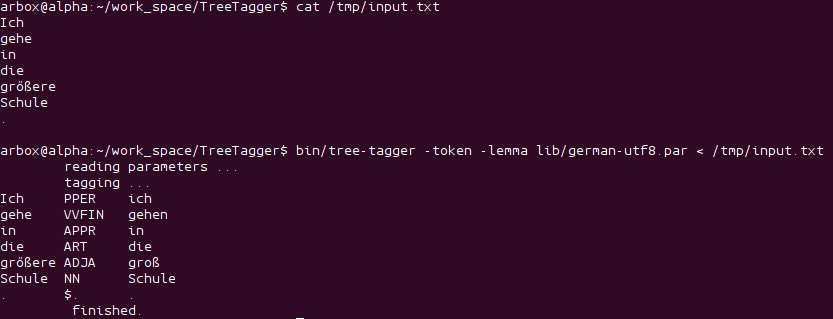
\includegraphics[width = \textwidth]{tree_tagger}
  \end{figure}
\end{frame}

\begin{frame}
  \frametitle{Nicht überwachte Methoden}

  %\textcite{biemann_unsupervised_2009}
\end{frame}

\begin{frame}[allowframebreaks]
  \nocite{*}
  \printbibliography
\end{frame}

\frame{
  Weiter mit Folien von Michael Collins.
}
\end{document}

%%% Local Variables: 
%%% mode: latex
%%% TeX-master: "main.presentation"
%%% End: 
